\Chapter{Keresztfordítás}

\Section{Formális nyelvek}

A keresztfordítás elméleti hátterét a formális nyelvek témaköre adja.
Ennek áttekintéséhez először be kell vezetni, az ábécé, a nyelv és nyelvtan fogalmát \cite{formalis}.
\begin{itemize}
\item Ábécének a szimbólumok tetszőleges, nem üres halmazát tekintjük, amelyet általában $\Sigma$-val jelölünk.
\item A $\Sigma$ ábécé feletti szavak egy tetszőleges $L$ halmazát az ábécéből alkotott (formális) nyelvnek nevezzük.
Az ábécé elemszámát és a szavak hosszát is általában végesnek tekintjük.
\item Azt a leírást, amellyel egy konkrét formális nyelvet megadhatunk, nyelvtannak nevezzük.
\end{itemize}

A nyelvtanokat két nagy csoportba sorolhatjuk, úgy mint generatív és analítikus nyelvtanok.
Egy generatív nyelvtan azt írja le, hogyan lehet előállítani az adott nyelvet egy adott szabályhalmazból.
Analítikus nyelvtanoknál az adott nyelv olvasási módját írjuk le, ugyancsak szabályokkal.

A generatív nyelvek osztályozása Noam Chomsky nyelvészhez köthető, aki az 1950-es években adta meg a nyelvek és nyelvtanok alapvető osztályait. Ezt az osztályozási módot nevezzük Chomsky-hierarchiának. Az egyes nyelvosztályokat 0-tól kezdődően egész számokkal jelölte. A 4 szintű hierarchiában a 0-ás a legáltalánosabb osztály, míg a 3-as a leginkább speciális. Ezek a következők.

\bigskip

\noindent \textbf{0. nyelvosztály}

\medskip

\begin{tabular}{ll}
\textbf{nyelvtan/nyelv} & Rekurzívan megszámlálható \\
\textbf{automata} & Turing-gép \\
\textbf{produkciós szabály} & Nincs megkötés \\
\end{tabular}

\bigskip

\noindent \textbf{1. nyelvosztály}

\medskip

\begin{tabular}{ll}
\textbf{nyelvtan/nyelv} & Környezetfüggő \\
\textbf{automata} & Korlátos nem determinisztikus Turing-gép \\
\textbf{produkciós szabályok} & $\alpha A \beta \rightarrow \alpha \gamma \beta$ \\
\end{tabular}

\medskip

Az 1. nyelvosztályt a környezetfüggő nyelvek osztályának nevezzük, ezt mutatja a produkciós szabály formája is.
Az $\alpha A \beta \rightarrow \alpha \gamma \beta$, azaz a leírás szabálya a $A \rightarrow \gamma$, de ez csak az $\alpha \rightarrow \beta$ környezetben alkalmazható.

\bigskip

\noindent \textbf{2. nyelvosztály}

\medskip

\begin{tabular}{ll}
\textbf{nyelvtan/nyelv} & Környezetfüggetlen \\
\textbf{automata} & Nem determinisztikus veremautomata \\
\textbf{produkciós szabályok} & $A \rightarrow \gamma$ \\
\end{tabular}

\medskip

A 2 nyelvosztályban található nyelvtanok szabály szerint az A -> $\gamma$, ahol a $\gamma$ tetszőleges jelsorozat, mely terminális és nemterminális szimbólumokat is tartalmazhat. Az A pedig egy itt is egy nemterminális szimbólum lesz.

\bigskip

\noindent \textbf{3. nyelvosztály}

\medskip

\begin{tabular}{ll}
\textbf{nyelvtan/nyelv} & Reguláris \\
\textbf{automata} & Véges determinisztikus automata \\
\textbf{produkciós szabályok} & $A \rightarrow a, A \rightarrow aB, A \rightarrow Ba$ \\
\end{tabular}

\medskip

A hierarchia 3. nyelvosztályába tehát olyan nyelvtanok tartoznak, melyek bal oldala mindig egy nemterminális szimbólum, a jobb oldala pedig vagy egy nemterminális szimbólum, vagy egy terminális és nemterminális szimbólum által alkotott sor.

\SubSection{Véges automaták és reguláris nyelvek}

Fontos szót ejteni a véges automatákról (\textit{Final State Machine}, FSM). A véges automaták olyan automaták, melyek meghatározott véges állapothalmaz, bemeneti ábécé, kezdő- és végállapot valamint átmeneti függvény megadása után egy rendszert képez. Ez felírható egy irányított gráffal, amelyben az egyes állapotok a gráf csúcspontjai. Mivel véges automatáról van szó, az automata az egyik állapotból egy input hatására egy másik állapotba kerül. Minden pillanatban pontosan egy adott állapot van érvényben.

Két nagy csoportot különböztetünk meg, úgy mint a determinisztikus és a nem determinisztikus automatákat.
A determinisztikus automaták esetében adott input és adott állapot esetében minding determinisztikus módon meghatározható, hogy melyik lesz a következő állapot. Ez a nemdeterminisztikus automatákra nem teljesül.

A keresztfordítás, és úgy általában a programozási nyelvek szempontjából azért érdemes a véges automatákkal foglalkoznunk, mert ezeknek a nyelvei tipikusan reguláris nyelvek, amelyek véges állapotú automatákkal reprezentálhatók.

\Section{Nyelvtanok definiálási módjai}

Az előző szakaszokban az egyes nyelvtanok osztályozási módját, azok fő jellemzőit tekinthettük át.
Most azt vizsgáljuk meg, hogy hogyan definiálhatunk egy konkrét reguláris nyelvet.
A programok leírásához hasonlóan ehhez is rendelkezésre állnak szöveges, és grafikus leírási módok.
Ez nyilvánvalóan a véges automaták és a reguláris nyelvek közötti szoros kapcsolatnak tudható be.
Reguláris nyelvek esetében a kibővített Backus-Naur formát (\textit{Extended Backus-Naur Form}, EBNF) a leginkább elterjedt leírási mód, míg ha véges állapotú automataként tekintünk a nyelvtanra, akkor például szintaxis diagram formájában is definiálhatjuk a nyelvtan. (Ez utóbbit szokták \textit{railroad} diagramna is nevezni.)

\SubSection{Kibővített Backus-Naur forma}

A Backus-Naur forma egy formális nyelvek leírására használható metanyelv, melyet John Backus hozott létre és mutatott be. Maga a metanyelv valójában szabályok halmaza, melyben terminális és nemterminális elemek találhatók meg adott összerendelésben, azaz kifejezésben melynek bal és jobb oldalán egy-egy elem áll általában \texttt{::=} vagy \texttt{:} jellel összekapcsolva \texttt{;}-vel lezárva a kifejezést \cite{ebnf}.

A terminális elemek olyan nyelvi elemek, melyek előre definiáltak, mint például a literálok (például szöveg- és szám literál).
A terminális elemeket a fentebb említett kifejezések bal oldalán nem jelennek meg.
A nem terminális kifejezések ezekből a terminális kifejezésekből, más nemterminális kifejezésekből, vagy ezek kapcsolataiból állnak. Tekintsük például az alábbi két definíciót.
\begin{cpp}
id ::= STRING;
integer ::= INT;
\end{cpp}
Az fentebb látható esetekben a kifejezések bal oldalán egy-egy nemterminális kifejezés áll, a jobb oldalon ezzel szemben terminális kifejezés, string, illetve integer literál áll. Az alább látható kifejezésben ezután felhasználhatjuk a már definiált elemeket is.
\begin{cpp}
sum ::=	integer "+" integer;
\end{cpp}
Megadhatók a kifejezések olyan módon is, hogy egy bal oldalon álló nemterminális kifejezés több módon is előállítható. Ilyenkor a jobb oldalon álló kifejezéseket \texttt{|} jellel, azaz \textit{vagy} kapcsolattal kell elválasztani. Emellett megadható benne idézőjelek között álló konkrét string is.

\begin{cpp}
sum ::= integer "+" integer;
neg ::= integer "-" integer;
mul ::= integer "*" integer;
summul ::= "(" integer + integer ")" * integer;
count ::= sum | neg | mul | summul;
\end{cpp}

A kibővített Backus-Naur forma az előbbi nyelvezet egy kiterjesztése \cite{scowen1998extended}.
Ebben a formális nyelv még pontosabb leírását segítő elemek jelentek meg, melyek közül a legfontosabbakat említjük itt meg.

A nyelv leírásában használhatjuk a \texttt{[} kifejezes \texttt{]} alakot, mely esetben a szögletes zárójelpárba írt kifejezések opcionálisak, nem kötelezően megjelenő elemek a szabályok alkalmazásakor.
Lehetőségünk van jelezni, hogy egy adott szerkezetben egy vagy több elem ismétlődhet. Ezt a \texttt{\{} elem \texttt{\}} kifejezéssel tehetjük meg, mely jelentése az adott elem nulla vagy többszöri megjelenése.
Emellett a zárójelpárba írt elemek csoportosíthatók azaz jelölhető például egy adott szabályban, hogy több különféle kifejezésre illeszkedhet, például
\begin{cpp}
math ::= integer ("+" | "-" | "*" | "/" ) integer
\end{cpp}
A fenti példában tehát a szabály olyan esetekre illeszkedik amikor két integer jelenik meg, viszont a közöttük lévő jel a \texttt{+}, a \texttt{-}, a \texttt{*} és a \texttt{/} bármelyike lehet.

\SubSection{Szintaxis diagramok}

A szintaxis diagramok a véges állapotú automaták leírásának egy, a nyelvek leírása szempontjából kedvezőbb leírási módját jelentik. Gyakran hivatkoznak rá \textit{railroad} diagramként is, mivel a gráf éleinek csatlakozási módja a sínekhez hasonlóan nyíl nélkül is képes jelezni azt, hogy mely irányba lehetséges átmenet, és mely irányba nem. A jelölési mód könnyen olvasható, külön formális definíciót nem igényel. A későbbiekben, a saját programozási nyelv definiálásánál majd láthatunk példát a használatára.

\Section{A feldolgozás lépései}

\Aref{fig:process}. ábrán láthatóak a fordítás főbb lépései.
\begin{figure}
\centering
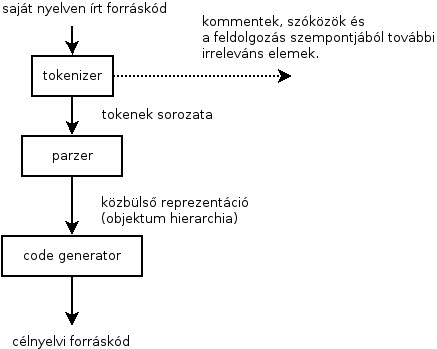
\includegraphics[scale=1]{kepek/process.png}
\caption{A keresztfordítás lépései}
\label{fig:process}
\end{figure}
A fordítók és értelmezők működéséről, azok megvalósítási módjáról teljeskörű útmutatásokat találhatunk a fellelhető irodalmakban \cite{compilers}.
A következő szakaszokban az általános lépéseknek a részletes bemutatására kerül majd sor.

\SubSection{Tokenizálás}

Az tokenizálás a fordítás első fő fázisa. A felhasználó által megadott programkód beolvasását követően a nyelvi feldolgozó azt tokenek sorozatára bontja.
A token egy, a karakternél magasabb szintű logikai egységet jelöl.
A feldolgozást végző egységet ebben a fázisban angol terminológia szerint \textit{tokenizer}-nek vagy \textit{lexer}-nek (esetenként \textit{scanner}-nek) szoktak nevezni.
A tokenizer minden elemhez hozzá kell tudjon rendelni a program egy tokent, mivel a későbbi feldolgozási lépések során már csak ezek kerülnek figyelembevételre.

A tokenek sorozatában általában nem szerepelnek a különböző fehér karakterek, mint például a szóköz, újsor, tabulátor karakterek.
Ezek általában szemantikai jelentéssel nem bírnak, a kód olvashatóságát segítik.

A tokenek definiálásához a karakterek halmaza felett definiálhatunk reguláris kifejezéseket.
A leggyakrabban előforduló tokenek típusok
\begin{itemize}
\item szám literál: \texttt{[0-9\_]+}
\item szöveg literál: \texttt{[a-zA-Z0-9\_]+}
\item zárójelek: \texttt{(} és \texttt{)}
\item fehér karakterek: \verb$(\n | \r | \r | \f | \t)+$
\end{itemize}

A tokenizálás a nyelvi feldolgozás egy tipikus feladata.
Emiatt már számos olyan program elérhető, amely segíti ezen programrész elkészítését.
Ezeket lexer, tokenizer vagy scanner generátoroknak nevezzük.
A generátoroknak meg kell adni egy szintaktikai leírást, mely alapján a lexert létrehozzák, azonban figyelni kell arra, hogy az adott generátornak megfelelő módon, és az általunk megadott nyelvre illeszkedő kifejezéseket adjunk meg.

A fellelhető generátorok közül azok használata tünt szerencsésebbnek, amelyek a reguláris kifejezések segítségével adják meg a feldolgozási elemeket. Ilyenek például az \textit{AnnoFlex}, \textit{JFlex} programok, ezekről részletesebben a szintaktikai elemzéssel foglalkozó fejezetben esik szó.

\SubSection{Nyelvi feldolgozás, parzolás}

A tokenek sorozata átkerül a feldolgozás következő lépéseként a parserhez.
A parzer és a tokenizer között a különbség elsősorban a feldolgozás absztrakciós szintjében van.
A parzolási folyamat szintén tipikus feladatnak tekinthető, ezért ahhoz is rendelkezésre állnak generátorok.
E mellett definiálhatunk saját rekurzív parzert is.

A lexer generátorokhoz hasonlóan a parzer generátorból is több elérhető program rendelkezésre áll.
Fontos megjegyezni, hogy olyan parzer és lexer generátort érdemes választani, melyek a lehető legjobban együtt tudnak műküdni.
Ilyen például a \textit{JFlex} és a \texttt{CUPS} generátor, mely generátort úgy terveztek, hogy egymással együttműködve tudnak működik.
A dolgozathoz elkészített program szempontjából ez a tervezettnél több problémát okozott.
Ez elsősorban a generátor programok verzióinak egyeztetéséből, és a nem túl naprakész dokumentációból adódott.

A nyelvi feldolgozás eredményeképpen egy objektum-hierarchia jön létre.

\SubSection{Kód generálás}

A keresztfordítás utolsó lépése az, hogy az objektum-hierarchierarchiából ismét egy szöveges leírási mód jöjjön létre (már a cél programozási nyelven). A konvertálás tulajdonképpen abból áll, hogy a hierarchiában szereplő objektumok az adott programozási nyelvnek megfelelően tudják visszaadni magukat szöveges formában.
